
 \FloatBarrier
\section{Multi-population Games}\label{sec:multi-pop}




\subsection{Matching pennies}

We implement a matching pennies game defining a society $\pop = \{p_1, p_2\}$ with two populations and two strategies per population, namely \emph{heads} and \emph{tails}. First, note that the payoff of the game in normal form is
%
\begin{table}[H]
\centering
 \begin{tabular}{|c|c|} \hline
  2, 1 & 1, 2 \\ \hline
  1, 2 & 2, 1 \\ \hline
 \end{tabular}
\end{table}
%
Now, the fitness vector of the  population $p_j$ can be expressed as $F^{p_j}(x^{p_k}) = A^{p_j} x^{p_k}$, for $p_j, p_k \in \pop$ and $p_j \neq p_k$. That is, the payoff of a population is affected only by the state of the opponent population.
The payoff matrices are defines as follows
%
\begin{equation}
  A^1 = \begin{pmatrix}
2 & 1 \\
1 & 2 
  \end{pmatrix}
\end{equation}
%
\begin{equation}
  A^2 = \begin{pmatrix}
  1 & 2 \\
  2 & 1 
  \end{pmatrix}
\end{equation}
%
Fig. \ref{fig:mp_game_rd} to \ref{fig:mp_game_logit} show the evolution of the social state with the evolutionary dynamics presented in Section \ref{sec:protocols}. 

\begin{figure}[h]
  \centering
  \begin{subfigure}[b]{0.45\textwidth}
	  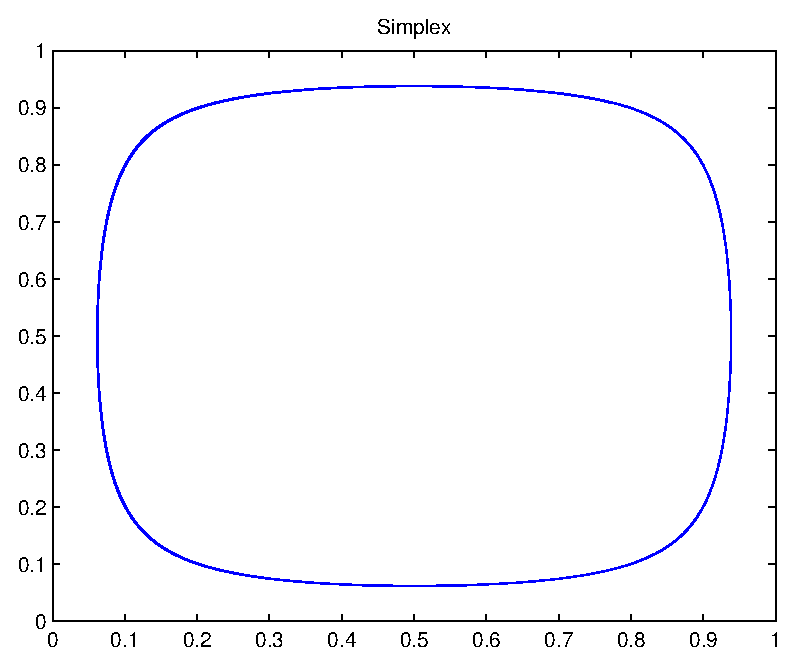
\includegraphics[width=\textwidth]{./images/test2_simplex_rd.eps}
	  \caption{Simplex.}
	  \label{fig:test2_simplex_rd}
  \end{subfigure}
  ~ 
  \begin{subfigure}[b]{0.45\textwidth}
	  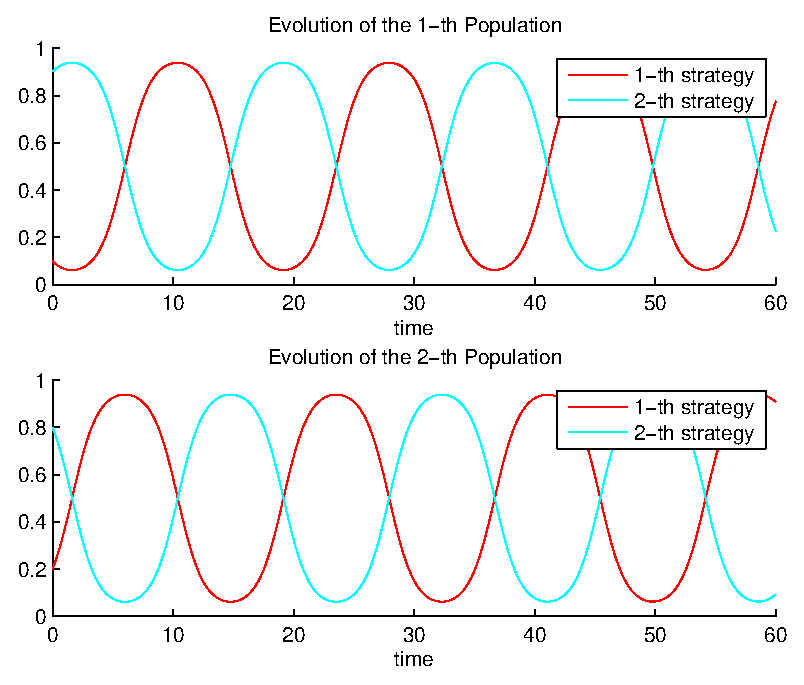
\includegraphics[width=\textwidth]{./images/test2_ev_rd.eps}
	  \caption{Evolution of the strategies in time.}
	  \label{fig:test2_ev_rd}
  \end{subfigure}
  \caption{Matching pennies game with replicator dynamics.}
  \label{fig:mp_game_rd}
\end{figure}



\begin{figure}[h]
  \centering
  \begin{subfigure}[b]{0.45\textwidth}
	  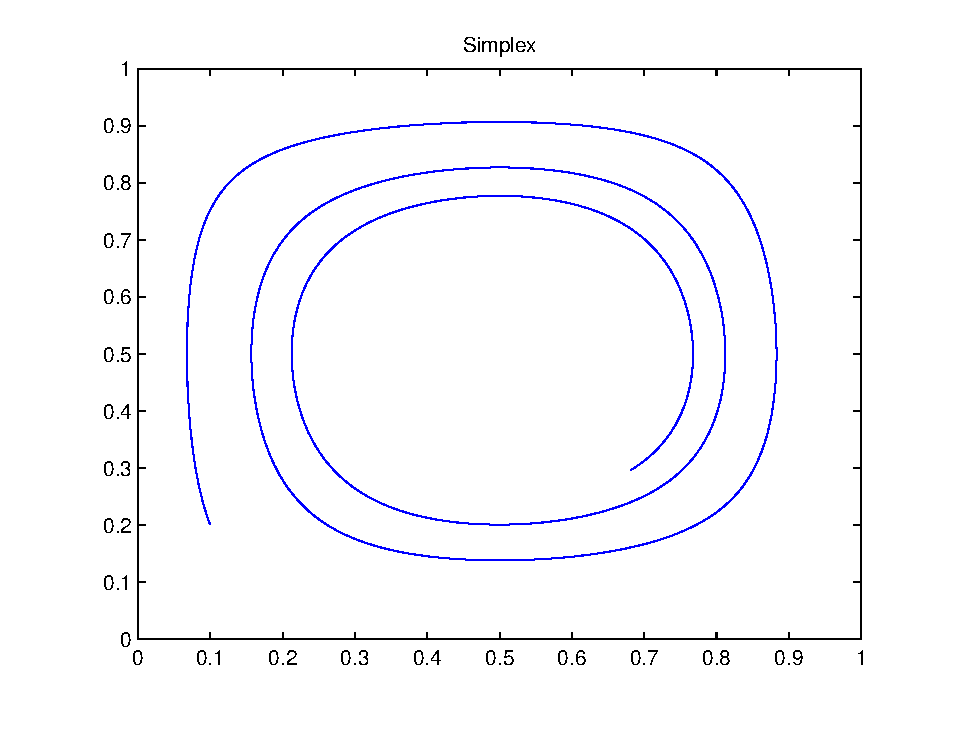
\includegraphics[width=\textwidth]{./images/test2_simplex_maynard_rd.eps}
	  \caption{Simplex.}
	  \label{fig:test2_simplex_maynard_rd}
  \end{subfigure}
  ~ 
  \begin{subfigure}[b]{0.45\textwidth}
	  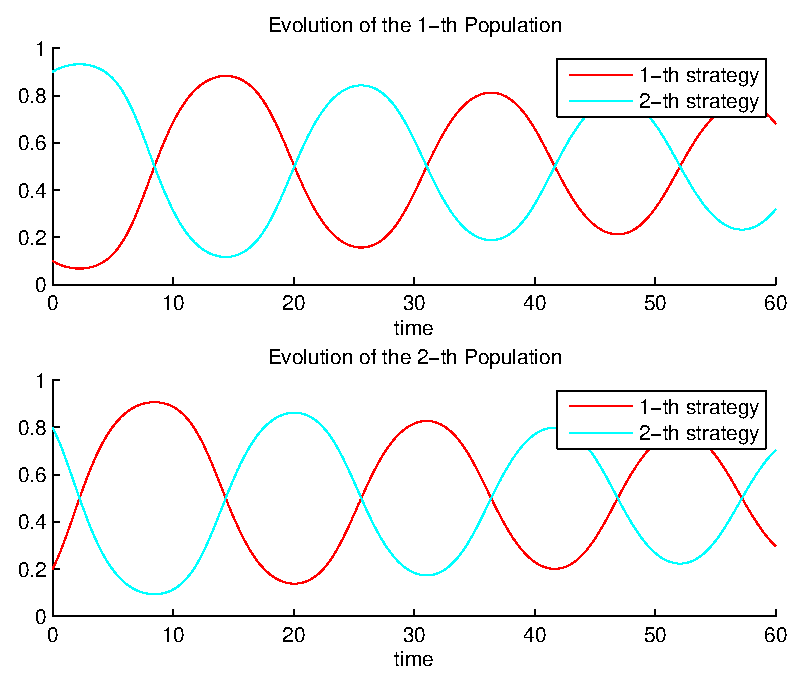
\includegraphics[width=\textwidth]{./images/test2_ev_maynard_rd.eps}
	  \caption{Evolution of the strategies in time.}
	  \label{fig:test2_ev_maynard_rd}
  \end{subfigure}
  \caption{Matching pennies game with Maynard replicator dynamics.}
  \label{fig:mp_game_maynard_rd}
\end{figure}



\begin{figure}[h]
  \centering
  \begin{subfigure}[b]{0.45\textwidth}
	  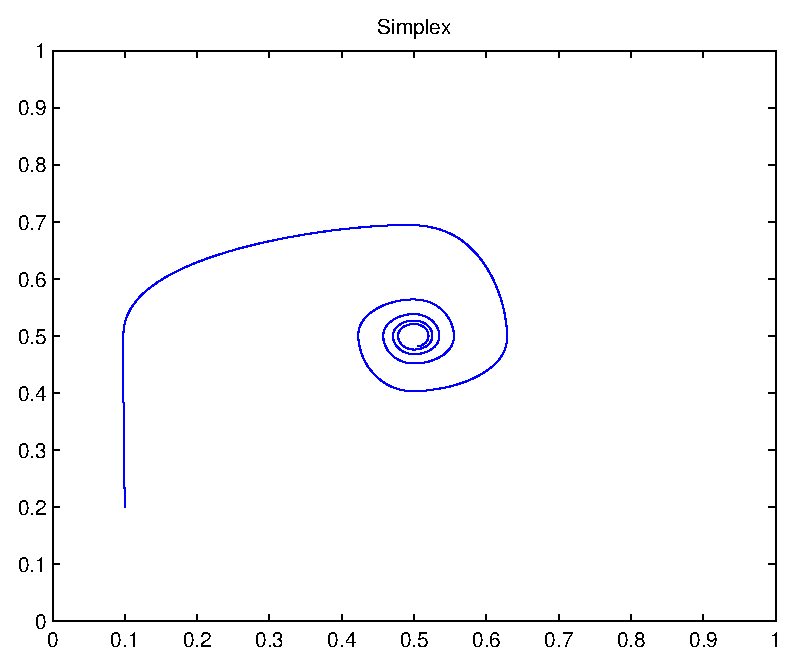
\includegraphics[width=\textwidth]{./images/test2_simplex_bnn.eps}
	  \caption{Simplex.}
	  \label{fig:test2_simplex_bnn}
  \end{subfigure}
  ~ 
  \begin{subfigure}[b]{0.45\textwidth}
	  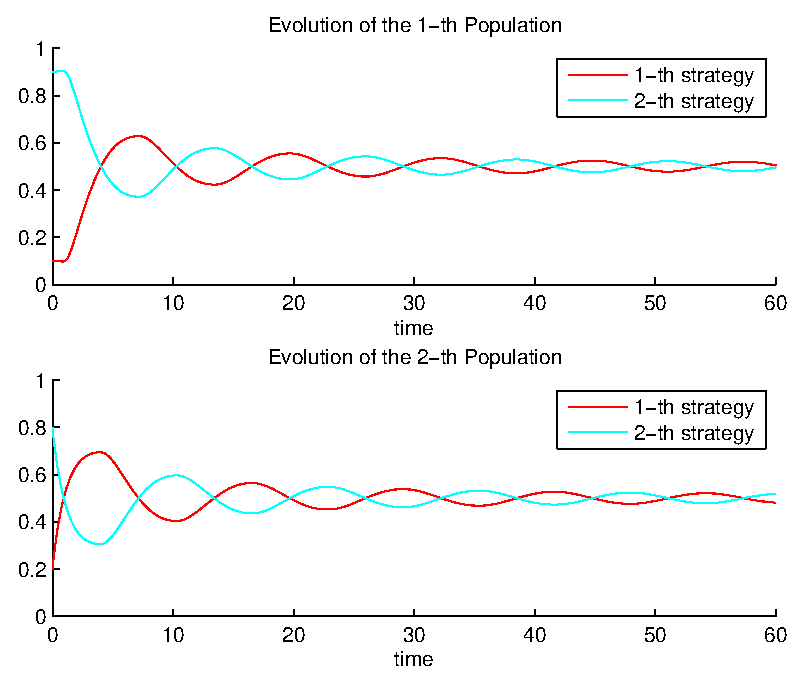
\includegraphics[width=\textwidth]{./images/test2_ev_bnn.eps}
	  \caption{Evolution of the strategies in time.}
	  \label{fig:test2_ev_bnn}
  \end{subfigure}
  \caption{Matching pennies game with BNN dynamics.}
  \label{fig:mp_game_bnn}
\end{figure}



\begin{figure}[h]
  \centering
  \begin{subfigure}[b]{0.45\textwidth}
	  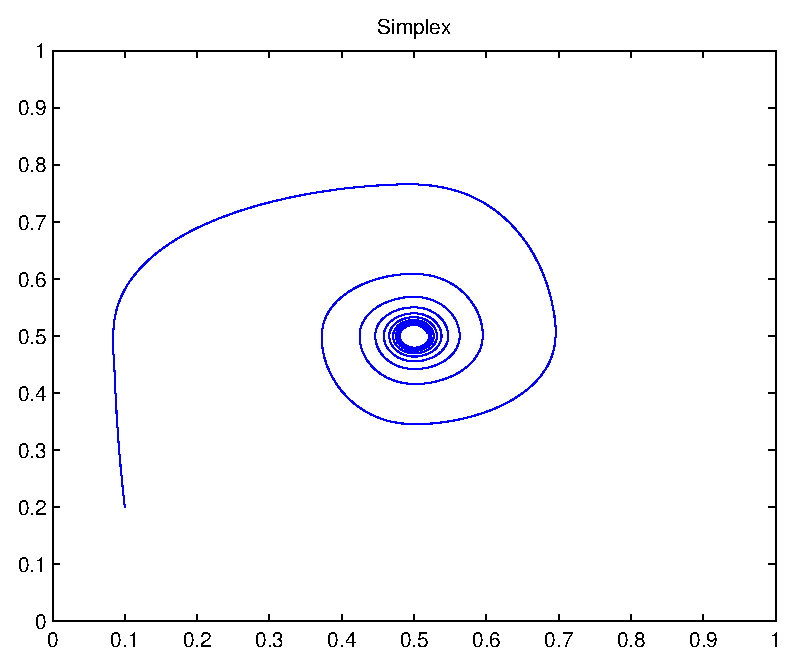
\includegraphics[width=\textwidth]{./images/test2_simplex_smith.eps}
	  \caption{Simplex.}
	  \label{fig:test2_simplex_smith}
  \end{subfigure}
  ~ 
  \begin{subfigure}[b]{0.45\textwidth}
	  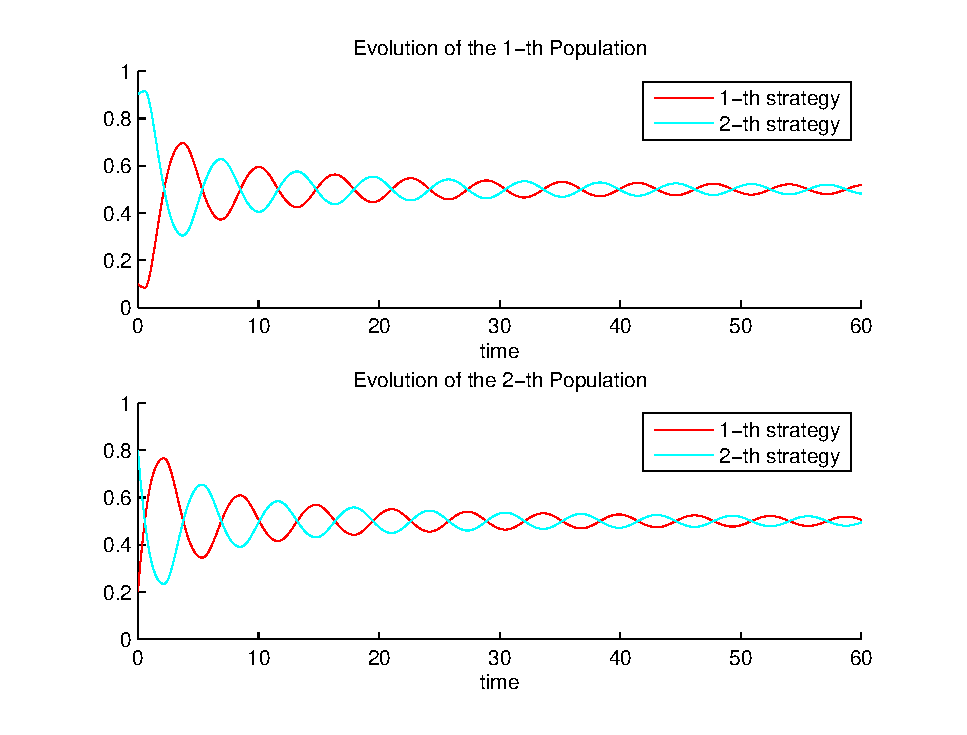
\includegraphics[width=\textwidth]{./images/test2_ev_smith.eps}
	  \caption{Evolution of the strategies in time.}
	  \label{fig:test2_ev_smith}
  \end{subfigure}
  \caption{Matching pennies game with Smith dynamics.}
  \label{fig:mp_game_smith}
\end{figure}



\begin{figure}[h]
  \centering
  \begin{subfigure}[b]{0.45\textwidth}
	  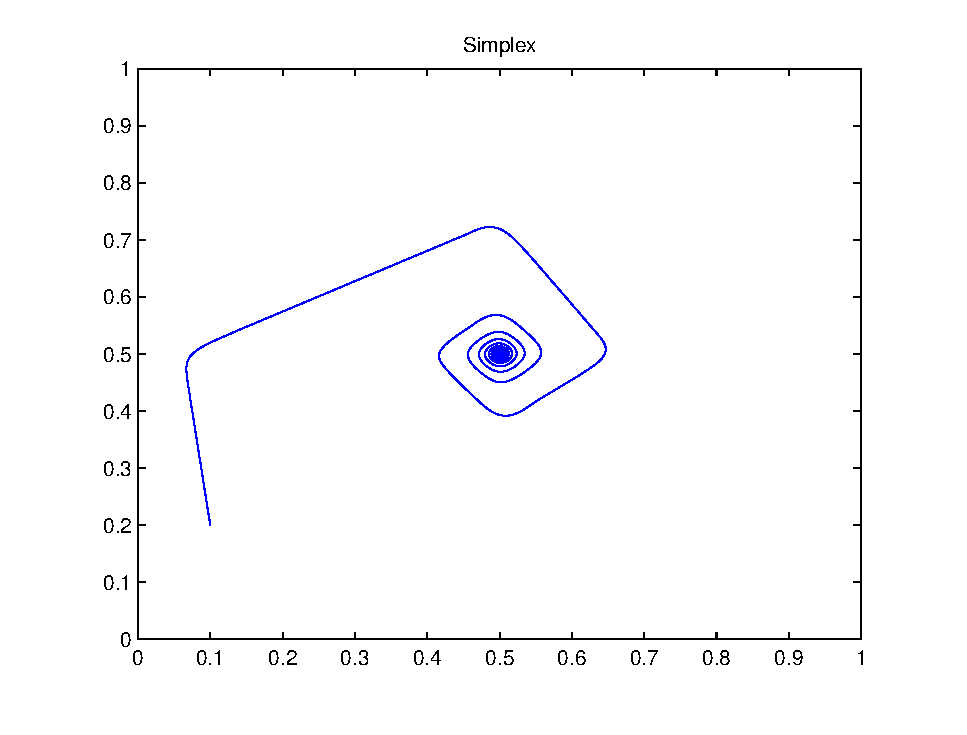
\includegraphics[width=\textwidth]{./images/test2_simplex_logit.eps}
	  \caption{Simplex.}
	  \label{fig:test2_simplex_logit}
  \end{subfigure}
  ~ 
  \begin{subfigure}[b]{0.45\textwidth}
	  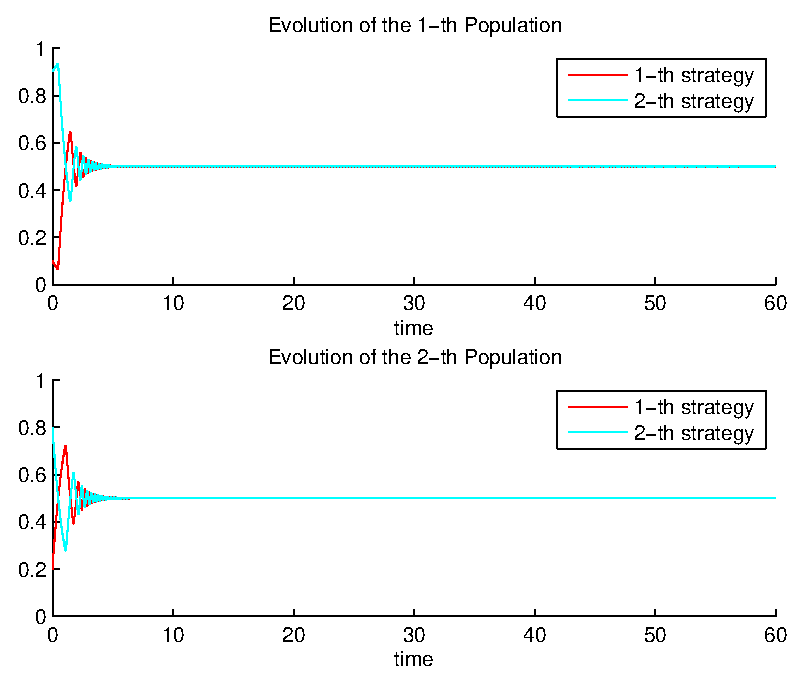
\includegraphics[width=\textwidth]{./images/test2_ev_logit.eps}
	  \caption{Evolution of the strategies in time.}
	  \label{fig:test2_ev_logit}
  \end{subfigure}
  \caption{Matching pennies game with Logit dynamics with $\eta=0.02$.}
  \label{fig:mp_game_logit}
\end{figure}

